% Copyright (c) 2026 Tomás Henao

\begin{example}
\textbf{Ejercicio:} Sea $f:S\longrightarrow T$ una función. % [cite: 927, 928, 929]
Supongamos que $(S, d_S)$ y $(T, d_T)$ son espacios métricos. % [cite: 929, 930, 931]
Si $Y \subseteq T$, entonces $X=f^{-1}(Y) \Leftrightarrow f(f^{-1}(Y))\subseteq Y$. % [cite: 933, 937, 938]
Si $X \subseteq S$ y $Y=f(X)$, entonces $X\subseteq f^{-1}(Y)$ y $X \subseteq f^{-1}(f(X))$. % [cite: 931, 940, 941, 943, 944]
Además, $f^{-1}(Y^{c})=(f^{-1}(Y))^{c}$. % [cite: 946]
En efecto, $x\in f^{-1}(Y^{c})$ sii $f(x)\in Y^{c}$ sii $f(x)\notin Y$ sii $x\notin f^{-1}(Y)$. % [cite: 946, 947, 948]
\end{example}

\begin{teorema}
Sea $f: A \to Y$. $f$ es continua en $A$ si y solo si para todo $C \subseteq Y$ cerrado, $f^{-1}(C)$ es cerrado en $A$. % [cite: 949, 950, 951, 959, 960, 964]
\end{teorema}

\begin{dem}
($\implies$) Supongamos que $f$ es continua en $A$. % [cite: 953, 957, 958, 959]
Sea $C \subseteq Y$ cerrado. Entonces $C^{c}$ es abierto en $Y$. % [cite: 964, 965, 966, 970, 974]
Por el teorema anterior, $f^{-1}(C^{c})$ es abierto en $A$. % [cite: 976, 977, 979]
Como $f^{-1}(C^{c})=(f^{-1}(C))^{c}$, entonces el complemento es abierto en $A$. Luego $f^{-1}(C)$ es cerrado en $A$. % [cite: 978, 979, 986]

($\impliedby$) Sea $U$ un abierto en $Y$, luego $U^{c}$ es cerrado. % [cite: 980, 983, 986]
Por hipótesis $f^{-1}(U^{c})=(f^{-1}(U))^{c}$ es un cerrado en $A$. % [cite: 981, 984, 986, 989]
Por lo anterior, $f^{-1}(U)$ es abierto en $A$, por lo tanto $f$ es continua en $A$. % [cite: 990, 991, 993, 994, 995]
\end{dem}

\begin{teorema}
Sea $f:A\rightarrow Y$ continua en $A$ y $B\subseteq A$ compacto. Entonces $f(B)$ es un compacto de $Y$. % [cite: 996, 998, 999, 1005, 1008, 1009, 1010, 1011]
\end{teorema}

\begin{dem}
Sea $\mathcal{F} = \{U_i\}$ un cubrimiento abierto de $f(B)$. % [cite: 1000, 1013, 1015]
Como $U_i$ es abierto y $f$ es continua, entonces $f^{-1}(U_i)$ es abierto en $A$. % [cite: 1017, 1018]

\textbf{Afirmación:} $B\subseteq\bigcup f^{-1}(U_i)$. % [cite: 1019]
En efecto, sea $x\in B$, entonces $f(x)\in f(B)$. % [cite: 1020, 1028]
Como $\mathcal{F}$ es un cubrimiento, $f(x) \in U_i$ para algún $U_i \in \mathcal{F}$. % [cite: 1030, 1032]
Es decir, $x\in f^{-1}(U_i)$. Luego $x\in \bigcup f^{-1}(U_i)$. % [cite: 1031, 1033, 1035]

Por la afirmación anterior $\mathcal{G}=\{f^{-1}(U_i)\}$ forma un cubrimiento abierto para $B$. % [cite: 1037, 1038, 1041, 1042]
Como $B$ es compacto, existen $f^{-1}(U_1), \dots, f^{-1}(U_n) \in \mathcal{G}$ tales que $B\subseteq\bigcup_{i=1}^{n}f^{-1}(U_i)$. % [cite: 1039, 1043, 1044, 1045, 1046]

\textbf{Afirmación:} $f(B)\subseteq\bigcup_{i=1}^{n}U_i$. % [cite: 1047]
En efecto, sea $x\in f(B)$, entonces existe $y\in B$ tal que $x=f(y)$. % [cite: 1048, 1049, 1050, 1051]
Como $y \in \bigcup_{i=1}^{n}f^{-1}(U_i)$, entonces $y\in f^{-1}(U_j)$ para algún $j \in \{1, \dots, n\}$. % [cite: 1059, 1064]
Luego $x=f(y)\in U_j$, lo que implica que $x\in\bigcup_{i=1}^{n} U_i$. % [cite: 1060, 1061]
Por lo tanto, $f(B)$ es compacto. % [cite: 1058, 1062]
\end{dem}

\begin{remark}
Si $f:A\rightarrow Y$ es continua y $B\subseteq A$ compacto entonces $f(B)$ es cerrado y acotado. % [cite: 1063, 1066, 1067]
\end{remark}

\begin{definicion}
Sea $f:A\rightarrow \R^{k}$, con $A\subseteq (X,d)$. Decimos que $f$ es acotada en $A$ si existe un número positivo $M>0$ tal que $\|f(x)\|\le M$ para todo $x\in A$. % [cite: 1073, 1075, 1076, 1078, 1079, 1080, 1081, 1082]
\end{definicion}

\begin{teorema}
Sea $f:A\rightarrow \R^{k}$ una función de un espacio métrico $A\subseteq (X,d)$ en $\R^{k}$. Si $f$ es continua en $A$ y $B\subseteq A$ compacto, entonces $f(B)$ es acotada. (Ejercicio). % [cite: 1083, 1086, 1087, 1088, 1090, 1091, 1093, 1094]
\end{teorema}

\begin{teorema}
Sea $f:A\rightarrow \R$ una función continua y $B\subseteq A$ compacto. Entonces existen puntos $p, q \in B$ tales que $f(p)=\inf f(B)$ y $f(q)=\sup f(B)$. % [cite: 1095, 1098, 1099, 1100, 1102, 1104, 1107, 1108]
\end{teorema}

\begin{dem}
Como $B$ es compacto y $f$ es continua, entonces $f(B)$ es compacto en $\R$. % [cite: 1109, 1110, 1112, 1114]
Por lo tanto $f(B)$ es cerrado y acotado. % [cite: 1111, 1115, 1116, 1118]
Como $f(B) \subseteq \R$ y es acotado, sabemos que existen el ínfimo y supremo de $f(B)$. % [cite: 1119, 1121, 1124, 1127, 1136, 1137, 1143]
Sean $m=\inf f(B)$ y $M=\sup f(B)$. % [cite: 1129, 1139]
Para todo $x\in B$, $m\le f(x)\le M$. % [cite: 1142, 1152]
Usando la caracterización de ínfimo y supremo, para $\epsilon=\frac{1}{n}$, existen sucesiones $\{x_n\}\subseteq f(B)$ y $\{y_n\}\subseteq f(B)$ tales que $x_n\rightarrow m$ y $y_n\rightarrow M$. (Ejercicio). % [cite: 1143, 1144, 1145, 1148, 1150, 1153, 1154, 1155, 1157, 1158, 1159]
Como $f(B)$ es cerrado entonces $m\in f(B)$ y $M\in f(B)$; es decir, existen $p, q \in B$ tales que $m=f(p)$ y $M=f(q)$. % [cite: 1160, 1161, 1163, 1164, 1165, 1166, 1167, 1169]
\end{dem}

\begin{remark}
En el teorema anterior, como $f(p)\le f(x)\le f(q)$ para todo $x\in B$, entonces los números $f(p)$ y $f(q)$ se llaman respectivamente, los valores mínimo y máximo globales (o absolutos) en $B$. % [cite: 1170, 1172, 1174, 1176, 1177, 1178, 1180]
\end{remark}

\begin{teorema}[Teorema del valor extremo]
Sea $f:[a, b] \rightarrow \R$ una función continua en $[a, b]$, entonces $f$ alcanza su máximo y mínimo absoluto, es decir existen $p, q \in [a, b]$ tal que $f(p)=\min f(x)$ y $f(q)=\max f(x)$ para $x\in [a, b]$. % [cite: 1181, 1182, 1184, 1185, 1186, 1187, 1219, 1222, 1224, 1225, 1227, 1228, 1229]
\end{teorema}

\begin{center}
\begin{tikzpicture}
    % Ejes
    \draw (-2,0) -- (4,0);
    \draw (0,-2) -- (0,3);
    % Segmento de función
    \draw[red!70, thick] (0,0) -- (2,1.5) node[above left, text=red!70] {$f$};
    \draw[red!70, thick] (0,0) circle (2pt);
    \draw[red!70, thick] (2,1.5) circle (2pt);
    % Línea punteada
    \draw[dashed, gray] (2,1.5) -- (2,0);
\end{tikzpicture}
\end{center}

\begin{definicion}
1. Se dice que $p \in A$ es un punto de máximo absoluto de $f$ en $A$, si $f(x)\le f(p)$ para todo $x\in A$. Decimos que $f(p)$ es el valor máximo absoluto de $f$ en $A$. % [cite: 1192, 1194, 1196, 1200, 1201, 1202, 1203]

2. Decimos que $p \in A$ es un punto de mínimo absoluto de $f$ en $A$, si $f(p)\le f(x)$ para todo $x\in A$. Decimos que $f(p)$ es el valor mínimo absoluto de $f$ en $A$. % [cite: 1204, 1206, 1209, 1213, 1214, 1218, 1221]
\end{definicion}

\begin{example}
La función $f:(0,1)\rightarrow \R$, $f(x) = x$ es continua en $(0,1)$ (Ejercicio), pero $f$ no alcanza su máximo ni mínimo absoluto. % [cite: 1233, 1234, 1236, 1238, 1240, 1241, 1242, 1243, 1244, 1246, 1248]
\end{example}

\begin{example}
Considere la función indicadora. Sea $K=[0,1]$ compacto. % [cite: 1250, 1252, 1253]
$$f(x) = \begin{cases} 1, & \text{si } x \in \Q \\ 0, & \text{si } x \in \mathbb{I} \end{cases}$$
Sea $x\in \R$, como $\Q$ e $\mathbb{I}$ son densos en $\R$, existen sucesiones $q_n\rightarrow x$ y $r_n\rightarrow x$. % [cite: 1255, 1257, 1261, 1262, 1271, 1272]

\textbf{Caso 1:} Si $x\in \Q$, entonces $f(x)=1$, pero $\lim_{n\to\infty} f(r_n) = 0 \neq f(x)$. Luego $f$ no es continua en $x$. % [cite: 1275, 1276, 1277, 1288, 1291, 1295, 1296]

\textbf{Caso 2:} Si $x\in \mathbb{I}$, entonces $f(x)=0$, pero $\lim_{n\to\infty} f(q_n) = 1 \neq f(x)$. % [cite: 1297, 1298, 1302]

Por lo anterior $f$ es discontinua en todo $\R$. % [cite: 1299, 1304, 1306]
\end{example}

\begin{teorema}
Sea $f:A\longrightarrow Y$ una función inyectiva y continua. Si $A$ es compacto, entonces $f^{-1}: f(A) \to A$ es continua. % [cite: 1307, 1309, 1310, 1311, 1314, 1329]
\end{teorema}

\begin{dem}
Dado que $f$ es inyectiva, la función inversa $f^{-1}: f(A) \to A$ está bien definida. % [cite: 1322, 1326, 1327, 1329, 1331]
Veamos que $f^{-1}$ es continua. Veamos que $(f^{-1})^{-1}(C) = f(C)$ mapea cerrados en cerrados. % [cite: 1324, 1332, 1333, 1342]
Sea $C \subseteq A$ cerrado en $A$. Como $A$ es compacto, $C$ es compacto. % [cite: 1336, 1338, 1339, 1345, 1350]
Como $f$ es continua, entonces $f(C)$ es compacto. Luego $f(C)$ es cerrado en $f(A)$. % [cite: 1346, 1352, 1353, 1354]
Luego $f^{-1}$ es continua. % [cite: 1355]
\end{dem}

\begin{example}
Considere la función $f:[0,2\pi)\longrightarrow S^{1}=\{(x,y)\in\R^{2} \mid x^{2}+y^{2}=1\} \subseteq \R^{2}$, % [cite: 1356, 1358, 1359]
dada por $\theta\mapsto f(\theta)=(\cos\theta, \mathrm{sen}\theta) = (f_1(\theta), f_2(\theta))$. % [cite: 1358, 1359, 1362, 1367]
\begin{center}
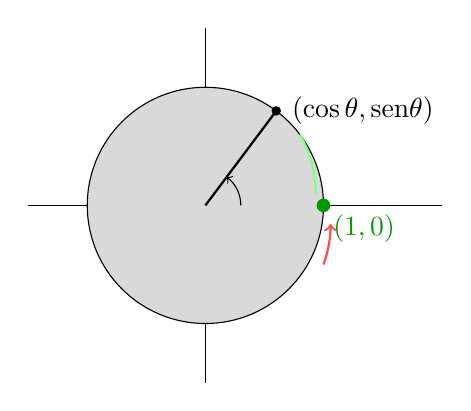
\begin{tikzpicture}[scale=1.5]
    % Ejes
    \draw (-1.5,0) -- (2,0);
    \draw (0,-1.5) -- (0,1.5);
    % Círculo relleno
    \draw[fill=gray!30] (0,0) circle (1cm);
    % Segmento y punto
    \draw[thick] (0,0) -- (0.6, 0.8) node[right, xshift=2pt] {$(\cos\theta, \mathrm{sen}\theta)$};
    \filldraw[black] (0.6, 0.8) circle (1pt);
    % Punto base
    \filldraw[green!60!black] (1,0) circle (1.5pt) node[below right, text=green!60!black] {$(1,0)$};
    % Arco rojo/verde (aproximación visual del trazo)
    \draw[->, red!70, thick] (1,-0.5) arc (-20:0:1cm);
    \draw[green!50, thick] (0.8, 0.6) arc (30:0:1cm);
    % Ángulo
    \draw[->] (0.3,0) arc (0:53:0.3);
\end{tikzpicture}
\end{center}

\textbf{Ejercicio 1:} $f$ es continua en $[0,2\pi)$ porque $f_1$ y $f_2$ son funciones continuas. % [cite: 1363, 1368, 1369, 1370, 1371]
\textbf{Ejercicio 2:} $f$ es biyectiva en $[0, 2\pi)$. % [cite: 1373, 1374, 1375, 1376, 1377]

Veamos que la función $f^{-1}:S^{1}\rightarrow [0,2\pi)$ no es continua en $(1,0)$. % [cite: 1378, 1379, 1381, 1383, 1384]
Considere la sucesión $x_n = 2\pi-\frac{1}{n} \in [0,2\pi)$ para todo $n \in \N$. % [cite: 1382, 1385, 1386, 1390]
$$ \lim_{n\rightarrow\infty}f(x_{n}) = \left(\lim_{n\rightarrow\infty}\cos\left(2\pi-\frac{1}{n}\right), \lim_{n\rightarrow\infty}\mathrm{sen}\left(2\pi-\frac{1}{n}\right)\right) = (1,0) $$ % [cite: 1388, 1389, 1393]
$$ \lim_{n\rightarrow\infty}f^{-1}(f(x_{n})) = \lim_{n\rightarrow\infty}x_{n} = \lim_{n\rightarrow\infty} \left(2\pi-\frac{1}{n}\right) = 2\pi $$ % [cite: 1396]
Pero $f^{-1}(1,0)=0 \neq 2\pi$. Por lo anterior, $f^{-1}$ es discontinua en $(1,0)$. % [cite: 1396]
\end{example}

\begin{teorema}
Sea $f: A \to \R$ una función continua en $c \in A$ tal que $f(c)\neq 0$. Entonces existe una bola $B(c,\delta)$ tal que $f(x)$ tiene el mismo signo de $f(c)$, para todo $x \in B(c,\delta)\cap A$. % [cite: 1397, 1398, 1399, 1402, 1403, 1404, 1406, 1408, 1410, 1411, 1412, 1413, 1415, 1416]
\end{teorema}

\begin{dem}
\textbf{Caso 1:} Si $f(c)>0$. Tomando $\epsilon=\frac{f(c)}{2}>0$, usando la definición de continuidad existe $\delta>0$ tal que: % [cite: 1417, 1419]
$f(x)\in B\left(f(c), \frac{f(c)}{2}\right)$ si $x\in B(c,\delta)\cap A$. % [cite: 1417, 1421]
Es decir, $|f(x)-f(c)| < \frac{f(c)}{2}$. % [cite: 1418, 1422]
Luego, $-\frac{f(c)}{2} < f(x)-f(c)$. % [cite: 1423]
Por tanto, $0 < \frac{f(c)}{2} = f(c)-\frac{f(c)}{2} < f(x)$ para todo $x\in B(c,\delta)\cap A$. % [cite: 1424, 1425, 1426, 1427]

\textbf{Caso 2:} Si $f(c)<0$. Tomando $\epsilon=-\frac{f(c)}{2}>0$, existe $\delta'>0$ tal que: % [cite: 1428, 1429, 1430, 1432]
$f(x)\in B(f(c),\epsilon)$ si $x\in B(c,\delta')\cap A$. % [cite: 1434]
Luego, $f(x)-f(c) < -\frac{f(c)}{2}$, lo que implica $f(x) < \frac{f(c)}{2} < 0$. % [cite: 1435, 1436]
Por lo anterior $f(x) < 0$. % [cite: 1437, 1438]
Luego, $f(x)$ tiene el mismo signo de $f(c)$, para todo $x\in B(c,\hat{\delta})$. % [cite: 1442, 1443, 1444, 1445, 1446]
\end{dem}

\begin{definicion}
\textbf{Homeomorfismo.} Sea $f:S\rightarrow T$ una función de un espacio métrico $(S, d_S)$ en $(T, d_T)$. % [cite: 1447, 1448, 1450]
Supongamos que $f$ es uno a uno en $S$. Luego $f^{-1}:f(S)\longrightarrow S$ está bien definida. % [cite: 1449, 1450]
Entonces diremos que $f$ es un homeomorfismo, si $f:S\rightarrow f(S)$ es continua y $f^{-1}:f(S)\rightarrow S$ es continua. % [cite: 1451, 1453, 1454, 1455, 1456]
\end{definicion}

\begin{example}
Los espacios métricos $\R$ y $(-\pi/2, \pi/2)$ con la métrica usual de subespacio de $\R$, son homeomorfos, porque la función $\tan: (-\pi/2, \pi/2)\rightarrow \R$ es un homeomorfismo. % [cite: 1459, 1460, 1461, 1463, 1465, 1467, 1468, 1469, 1470, 1471, 1474, 1475, 1476]
\end{example}